\documentclass{article}
\usepackage{graphicx}
\usepackage[a4paper, margin=2.5cm]{geometry}
\usepackage{parskip}
\usepackage{amsmath}
\usepackage{hyperref}
\usepackage{algorithm}
\usepackage{algpseudocode}

\begin{document}

\vspace*{3cm}

\begin{center}
    \LARGE \textbf{Relazione Progetto Algoritmi\\ e Strutture Dati} \\[1.5cm]
    
    \large
    Nassivera Filippo 165594 \\
    \texttt{165594@spes.uniud.it} \\[0.5cm]
    
    Viciguerra Francesco 166896 \\
    \texttt{166896@spes.uniud.it} \\[0.5cm]
    
    Rossetto Mattia 169423 \\
    \texttt{169423@spes.uniud.it} \\[0.5cm]
    
    \vspace{1cm}
    5 giugno 2025 \\[2cm]
    
    \includegraphics[width=0.3\textwidth]{Immagine1.png} \\
    \vspace{0.5cm}
    \textbf{}Università degli studi di Udine\\[0.5cm]
    \nolinkurl{https://github.com/BlackHole00/alg_e_str_dati_elaborato}
\end{center}

\thispagestyle{empty}  % ← niente numero in prima pagina
\newpage

\setcounter{page}{1} 
\tableofcontents

\newpage

\section{Introduzione}
    Il progetto richiede l’implementazione e la misura del rendimento di quattro algoritmi di ordinamento: \\
    quicksort, quicksort3way, countingsort ed un quarto algoritmo a scelta.
    
    Il quarto algoritmo da noi scelto è introsort.
    
    \subsection{Algoritmi di ordinamento}
        Questo tipo di algoritmi risolve un problema molto comune, ovvero:
        data una sequenza $a_1, a_2,\dots, a_n$ di interi, determinare una permutazione $\pi$ degli indici tale che $a_{\pi(1)} \le a_{\pi(2)} \le \dots \le a_{\pi(n)}$ (nel caso di un ordinamento in ordine crescente).

        In altre parole, un algoritmo di ordinamento riceve in input un vettore di elementi di dimensione n e restituisce in output lo stesso vettore, ma con gli elementi permutati come visto sopra.
        
        Il problema di ordinamento in sé non è complesso da risolvere, ma, come vedremo, è complesso trovare algoritmi che lavorano con efficienza e la mantengono al crescere di n.

    \subsection{Misurazione nel dettaglio}
        Viene richiesta l'implementazione di un programma per la misurazione dei tempi medi di esecuzione degli algoritmi, al variare della lunghezza $n$ dell'array e della dimensione $m$ del range di interi contenuta in esso.\\

        Segue quindi che verranno generati due set di dati, ovvero:
        \begin{itemize}
            \item Tempo medio al variare della lunghezza del vettore (n), con parametro m fisso.
            \item Tempo medio al variare della dimensione m, con parametro n fisso.
        \end{itemize}
        
        Notiamo inoltre che ogni set di dati è formato da 250 coppie di valori
        $$v_i = (n_i\text{ o }m_i, tempo\space medio)$$

        \subsubsection{Determinazione dei valori delle ascisse}
            Si è considerato opportuno ottenere 250 campioni per set.\\
    
            Le successioni dei valori $n_i$ e $m_i$ sono invece state generate dalla funzione esponenziale seguente (si consideri come esempio il calcolo di $n_i$):
            $$n_i=\lfloor A\cdot B^i\rfloor$$
            Dove $A$ e $B$ sono state opportunamente scelte in modo che $n_0=100$ e $n_{249}=100000$.\\
    
            Analogamente definiamo la successione $m_i$, con costanti $A$ e $B$ poste in modo che $m_0=10$ e $m_{249}=1000000$.

        \subsubsection{Cronometraggio del tempo medio}
            Il clock di sistema e le API fornite da molti sistemi operativi non permettono di calcolare il tempo di esecuzione in maniera precisa. Infatti, oltre al problema della sospensione dei processi, i clock hanno anche una risoluzione minima. Gli algoritmi, specialmente per variabili $n$ piccole possono terminare con velocità tale da non essere misurabile (ovvero al di sotto della risoluzione minima). Anche se un algoritmo terminasse con velocità percepibile vi sarebbero comunque errori di approssimazione.\\

            Per ovviare a questo problema, ogni misurazione viene ripetuta più volte, per calcolare poi il tempo medio, in modo da avere un errore relativo massimo pari a $0.001$.

        \subsubsection{Dinamicità del codice}
            Notiamo infine che tutte le costanti sopra indicate sono facilmente configurabili nel codice, in modo da facilitare la velocità di iterazione, di sviluppo e testing degli algoritmi e del progetto nella sua interità.

\section{Aspetti Implementativi}
    Il progetto è stato suddiviso in due componenti principali:
    \begin{itemize}
        \item \textbf{Runner}: esegue gli algoritmi e produce file \textit{CSV} interpretabili dal \textit{Visualizer}. È implementato in C, utilizzando esclusivamente la \textit{standard library}.
        \item \textbf{Visualizer}: legge i file \textit{CSV} e fornisce una visualizzazione interattiva dei grafici. È implementato in Python, mediante la libreria \textit{matplotlib}.
    \end{itemize}

    \subsection{Runner}
        Segue una descrizione dei principali aspetti implementativi del Runner.

        La generazione dei vettori disordinati è deterministica: ogni esecuzione del codice ordina gli stessi vettori. Ciò è stato ottenuto impostando un seme costante per il generatore pseudo-casuale tramite la chiamata a funzione \texttt{srand(0)}. In C, infatti, la generazione di numeri casuali è solo pseudo-casuale; di conseguenza, le successive chiamate a \texttt{rand()} producono sempre la stessa sequenza di valori.

        Un altro aspetto rilevante riguarda la misurazione dei tempi di esecuzione degli algoritmi: il cronometraggio esclude il tempo necessario all’inizializzazione del vettore da ordinare, in modo da ottenere una stima più accurata del solo tempo di ordinamento.

   \subsection{Collaborazione}
    L’intero progetto è stato sviluppato in modalità collaborativa tramite l’uso di \textit{Git} e \textit{GitHub}. La repository è disponibile a \href{https://github.com/BlackHole00/alg_e_str_dati_elaborato}{questo indirizzo}.

\section{Gli algoritmi}
    \subsection{Quicksort}
        Questo algoritmo mette in pratica l'idea di utilizzare l'ultimo elemento dell'array come perno e trovare la posizione che l'elemento avrebbe nel vettore ordinato.\\
        Una funzione chiamata partition si occupa di trovare il collocamento di \textit{p} e posizionando a sinistra di \textit{p} gli elementi minori o uguali a \textit{p} e a destra quelli maggiori.
        
        Dopo partition viene eseguita una chiamata ricorsiva a quicksort per ciascuno dei due sotto array, il tutto si ripete finché i sotto array non saranno di un singolo elemento, dunque già ordinati, a quel punto il vettore preso in input risulterà ordinato.
    
        \subsubsection{Complessità}
            Quicksort ha una complessità $\Theta(n^2)$ nel caso peggiore, ovvero se il vettore in input è ordinato al contrario o è già ordinato, di conseguenza il perno scelto è sbilanciato.
            
            Mentre nel caso medio e migliore si ha una complessità $\Theta(nlogn)$.\\
            Questa complessità deriva dall'operazione di partition, che trova l'indice in cui posizionare il perno, la quale ha complessità $\Theta(n)$ e dalle due operazioni di quick sort nei sotto array, che hanno ciascuna complessità $\Theta(logn)$.
            
            Si nota quindi che l'algoritmo tenderà ad essere meno efficiente per vettori composti da elementi appartenenti ad un range di valori piccolo, quindi con molti elementi ripetuti, in quanto ci si ricondurrebbe asintoticamente al caso peggiore.
            
            Infine, questo algoritmo è in-place, ma non è stabile.

    \subsection{Quicksort3way}
        Quest'algoritmo è una variante del quicksort, implementata per migliorare il costo nel caso peggiore.
        
        La peculiarità di questo algoritmo è il cambiamento alla modalità di partizionamento del vettore: quest'ultimo non viene più partizionato in due sotto array, ma in tre: gli elementi minori di \textit{p}, quelli uguali a \textit{p} e quelli maggiori.\\
        Verrà poi riapplicato ricorsivamente l'algoritmo nel sottoarray contenente gli elementi minori di \textit{p} e nel sottoarray contenente gli elementi maggiori di \textit{p}.

        \subsubsection{Complessità}
            Nel caso peggiore quest'algoritmo ha complessità $\Theta(n^2)$, ciò si verifica quando il vettore è già ordinato, di conseguenza il perno scelto è sbilanciato.\\
            Mentre nel caso medio e migliore ha complessità $O(nlogn)$.
            
            Notiamo che l'algoritmo non riesce a migliorare la complessità asintotica nel caso peggiore, tuttavia vi è un miglioramento nel caso il vettore abbia molti elementi duplicati, caso che il quicksort normale non riesce a gestire al meglio.
            
            L'algoritmo è in place, ma non è stabile.\\

    \subsection{CountingSort}   
        CountingSort è un algoritmo di ordinamento non basato su scambi e confronti. Segue quindi che è applicabile solo su un insieme ristretto di possibili array, più nel particolare, l'ordinamento è possibile solo se il vettore è costituito da interi nell'intervallo $[a, b]$.
        
        Verrà creato un vettore C di dimensione $m=b-a+1$ al cui interno verrà salvato il numero di volte che l'indice stesso compare nel vettore (C[0] conterrà quante volte $a$ compare nel vettore, C[1] lo farà per $a+1$ ecc.).
        
        Successivamente, partendo da $i=1$, si porrà $C[i]=C[i]+C[i-1]$, in modo che in $C[i]$ si abbia la posizione del primo termine $a+i$ trovato scorrendo il vettore.
        
        Sfruttando C si percorrerà il vettore di input da destra a sinistra, posizionando ogni elemento trovato nella posizione corretta (l'indice presente in $C[A[i]-a]$) in un vettore di output.

        \subsubsection{Complessità}        
            La complessità di countingsort è $\Theta(n + m)$, dove $m$ è la dimensione dell'intervallo contenente tutti gli elementi inseriti nell'array. Nello specifico: $$m = b - a + 1$$

            Segue che se $m = O(n)$, l'algoritmo da costo lineare, quindi asintoticamente preferibile agli algoritmi di ordinamento discussi in questo documento.

        \subsubsection{Scelte implementative}
            Prima di tutto notiamo che $a$ e $b$ non sono valori costanti conosciuti, invece vengono trovati a runtime facendo una scansione del vettore. Questo implica che il $C$ deve essere dinamicamente allocato, cosa che comporta un incremento del costo in termini di costanti moltiplicative, sebbene quello asintotico rimanga lo stesso.

            Si nota inoltre che non è stato implementato alcun algoritmo di caching o  riutilizzo della memoria dinamicamente allocata (necessaria per il vettore $C$ e per la copia del vettore in input). Ciò implica che il misuramento della performance dell'algoritmo include anche il costo della chiamata alle funzioni malloc e free.

            Sebbene sia possibile implementare soluzioni di gestione più intelligente della memoria (quali alla cosiddetta "Memory Arena", per esempio), che sarebbero in grado di annullare questo costo, questo comporterebbe una peggiore stabilità delle misurazioni, indesiderabile nel progetto attuale (ad esempio, alcune chiamate a counting sort, anche con lo stesso numero di elementi, potrebbero allocare memoria, mentre altre no).

    \subsection{Introsort}
        Introsort è un algoritmo di ordinamento ibrido, che utilizza i seguenti algoritmi:
        \begin{itemize}
            \item Quick Sort: generalmente molto efficiente, ma nel caso peggiore ha complessità $\Theta(n^2)$. Questo accade quando il vettore è già ordinato (o quasi ordinato), e il pivot scelto genera partizioni fortemente sbilanciate. Va notato che, per vettori piccoli, quicksort può comportarsi peggio in media rispetto a vettori più grandi, poiché una maggiore regolarità nei dati aumenta, causando l'incremento della probabilità di un partizionamento sfavorevole.
            \item Heap sort: sfruttando una struttura dati heap, consente di ordinare un vettore con complessità $\Theta(n \log n)$. Tuttavia, presenta una costante moltiplicativa più elevata rispetto a quicksort. Ne consegue che, per vettori di grandi dimensioni con bassa regolarità nei dati, quicksort risulta generalmente preferibile. Al contrario, heap sort può essere più vantaggioso su array di dimensioni contenute, soprattutto in presenza di una forte regolarità nei dati.
            \item Insertion sort: sebbene questo algoritmo abbia complessità asintotica $\Theta(n^2)$, presenta costanti moltiplicative molto basse. È quindi una soluzione efficiente per vettori di piccole dimensioni, ovvero quando la lunghezza è costante o molto ridotta.
        \end{itemize}

        Segue quindi la strategia implementata da introsort per sfruttare al meglio gli algoritmi precedentemente menzionati:
        \begin{itemize}
            \item Indipendentemente dal contesto, quando la lunghezza del vettore da ordinare è inferiore a una costante predefinita (solitamente 16 elementi), viene utilizzato insertion sort, che risulta particolarmente efficiente per array di piccole dimensioni.
            \item L’algoritmo applica inizialmente fino a $max\_depth = 2 \cdot \log_2(n)$ chiamate ricorsive di quicksort, sfruttando la sua efficienza sui dati di grandi dimensioni.
            \item Alla chiamata successiva, se la profondità ricorsiva supera $max\_depth$, l’algoritmo utilizza heap sort, a condizione che il sottovettore da ordinare abbia dimensione superiore alla soglia costante precedentemente definita. In caso contrario, si ricorre nuovamente a insertion sort.
        \end{itemize}

        \subsubsection{Pseudo Codice}
            Viene riportato lo pseudo codice di introsort:

            \begin{algorithm}[H]
                \caption{Introsort}
                \begin{algorithmic}
                    \Procedure{Introsort}{$A, n$}
                        \State $maxDepth \gets 2 \cdot \lfloor \log_2(n) \rfloor$
                        \State \Call{IntrosortUtil}{$A, 1, n, maxDepth$}
                    \EndProcedure
    
                    \Procedure{IntrosortUtil}{$A, start, end, depthLimit$}
                        \If{$end - start + 1 \leq 16$}
                            \State \Call{InsertionSort}{$A, start, end$}
                        \ElsIf{$depthLimit = 0$}
                            \State \Call{HeapSort}{$A, start, end$}
                        \Else
                            \State $pivot \gets$ \Call{Partition}{$A, start, end$}
                            \State \Call{IntrosortUtil}{$A, start, pivot - 1, depthLimit - 1$}
                            \State \Call{IntrosortUtil}{$A, pivot + 1, end, depthLimit - 1$}
                        \EndIf
                    \EndProcedure
                \end{algorithmic}
            \end{algorithm}
    
        \subsubsection{Complessità}
            Per capire la complessità dell'algoritmo è necessario analizzarne il costo delle singole modalità operative. Consideriamo dunque il caso peggiore.

            Poiché l’algoritmo \textit{heapsort} ha comportamento uniforme per qualunque input, concentriamoci sul caso peggiore del \textit{quicksort}. Supponiamo che il vettore in input sia già ordinato e di dimensione $n$, tale che l’albero delle chiamate ricorsive di Introsort sia completo (cioè $n = 2^m$ per qualche $m \in N$).
            
            Notiamo ora che l'algoritmo si comporta come quicksort solo per i primi $max\_depth$ livelli. Segue che partition verrà chiamato un numero limitato di volte: per ogni livello, verrà chiamato $2^i$ volte con ogni chiamata su $\lceil\frac{n - 2^{i - 1}}{2^i}\rceil$ elementi, dove $i$ è il livello corrente (i perni non vengono inclusi nella chiamata ricorsiva). Segue che il costo per livello, nel caso peggiore è:
                $$\Theta(2^i\cdot \frac{n - 2^{i - 1}}{2^i})=\Theta(n-2^{i-1})$$
            Siccome $i = O(max\_depth) = \Theta(log(n))$:
                $$\Theta(n-2^{i-1})=\Theta(n-O(log(n)))=\Theta(n)$$
            Segue che il costo complessivo delle chiamate a partition è:
                $$\sum_{i = 0}^{max\_depth - 1}{\Theta(n)}=\Theta(nlog(n))$$

            Analizziamo ora il costo necessario per terminare l'ordinamento del vettore utilizzando heapsort. Notiamo che verranno effettuate $2^{max\_depth}$ chiamate, ciascuna su $\lceil\frac{n-2^{max\_depth}}{2^{max\_depth}}\rceil$ elementi (come prima, vengono esclusi i perni). Segue che vi sarà un costo totale di:
                $$\Theta(2^{max\_depth}\cdot \frac{n-2^{max\_depth}}{2^{max\_depth}}log(\frac{n-2^{max\_depth}}{2^{max\_depth}}))=$$
                $$\Theta((n-2^{max\_depth})(log(n-2^{max\_depth})-log(2^{max\_depth})))=$$
                $$\Theta((n-log(n)(log(n-log(n))-log(n))=\Theta(nlog(n))$$

            Sommando quindi i contributi di \textit{quicksort} e \textit{heapsort} concludiamo dicendo che introsort ha complessità $\Theta(nlog(n))$ nel caso peggiore. Analogamente è anche possibile calcolare il costo nel caso medio e migliore che è $\Theta(nlog(n))$.

            Osserviamo infine che le eventuali chiamate ad insertionsort sono fatte per array di dimensione costante, quindi hanno costo asintotico $\Theta(c^2)=\Theta(1)$ costante. Nel nostro caso, ricordiamo, $c=16$. Il contributo complessivo di queste chiamate resta dunque trascurabile rispetto al termine dominante $\Theta(n \log n)$.

\section{Grafici}
    Di seguito sono riportati i grafici dei vari algoritmi ottenuti al variare della lunghezza dell'array $n$ o della dimensione $m$ del range di valori nell'array. Vengono presentati i risultati sia in scala lineare, che in scala logaritmica.
    
    \subsection{Quicksort}
        \subsubsection{Grafici al variare di \textit{n}}
            \begin{center}
                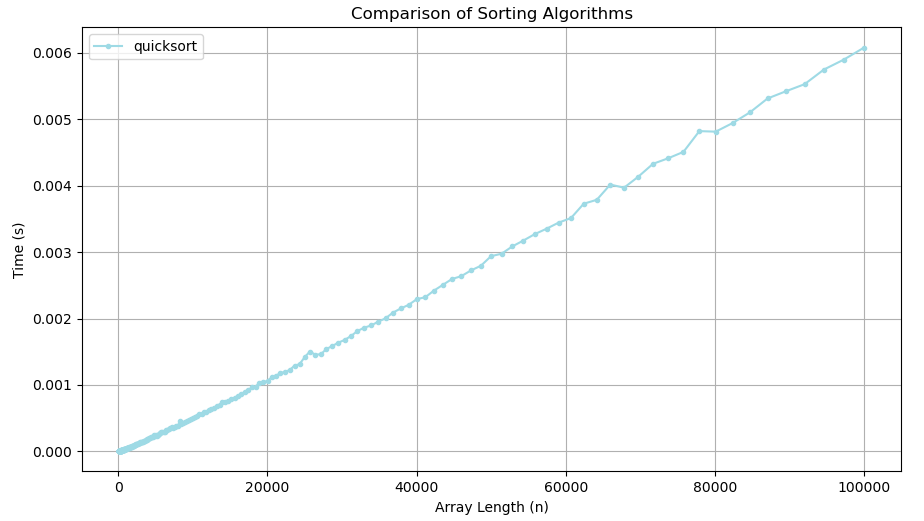
\includegraphics[width=0.6\textwidth]{Quicksort.png} \\
                %\vspace{0.5cm}
                \textbf{Grafico.1} Grafico in scala lineare\\
                \vspace{0.5cm}
                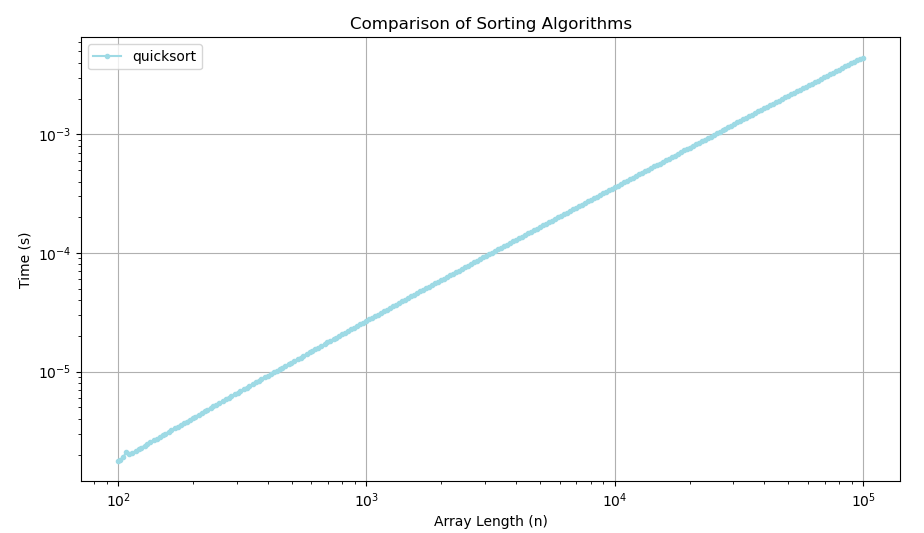
\includegraphics[width=0.6\textwidth]{Quicksort_Log.png} \\
                \textbf{Grafico.2} Grafico in scala logaritmica\\
            \end{center}
            Il comportamento dell'algoritmo al variare di $n$ non presenta particolari discrepanze con l'analisi asintotica.

        \subsubsection{Grafici al variare di \textit{m}}
            \begin{center}
                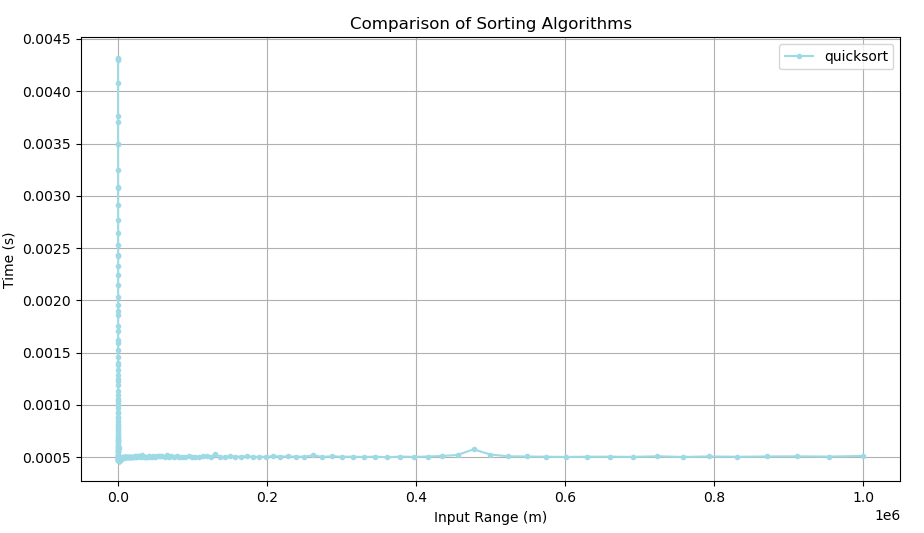
\includegraphics[width=0.6\textwidth]{Quicksort_InputRange.png} \\
                %\vspace{0.5cm}
                \textbf{Grafico.3} Grafico in scala lineare\\
                \vspace{0.5cm}
                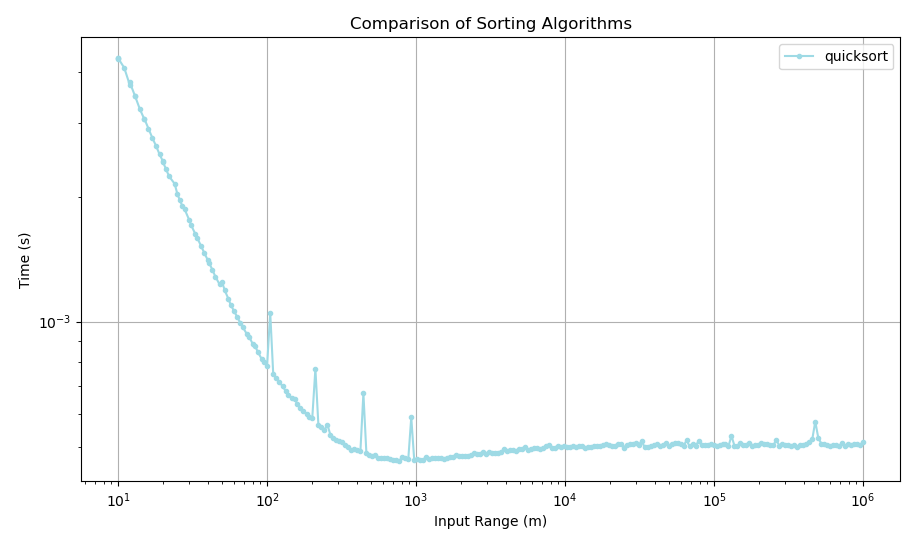
\includegraphics[width=0.6\textwidth]{Quicksort_InputRange_Log.png} \\
                \textbf{Grafico.4} Grafico in scala logaritmica\\
            \end{center}
            Come si può osservare, soprattutto nel grafico a scala logaritmica, più il range di valori è piccolo, più tempo impiega quicksort per l'ordinamento. Come abbiamo già detto in precedenza, se quicksort trova un vettore già ordinato, la sua complessità diventa quadratica. In questo caso più il range di valori è piccolo, più elementi uguali ci sono nel vettore e, dunque, il vettore risulta già parzialmente ordinato. Quicksort, nel particolare partition, attuerà una serie di operazioni che allungheranno solamente il processo di ordinamento.

    \subsection{Quicksort3way}
        \subsubsection{Grafici al variare di \textit{n}}
            \begin{center}
                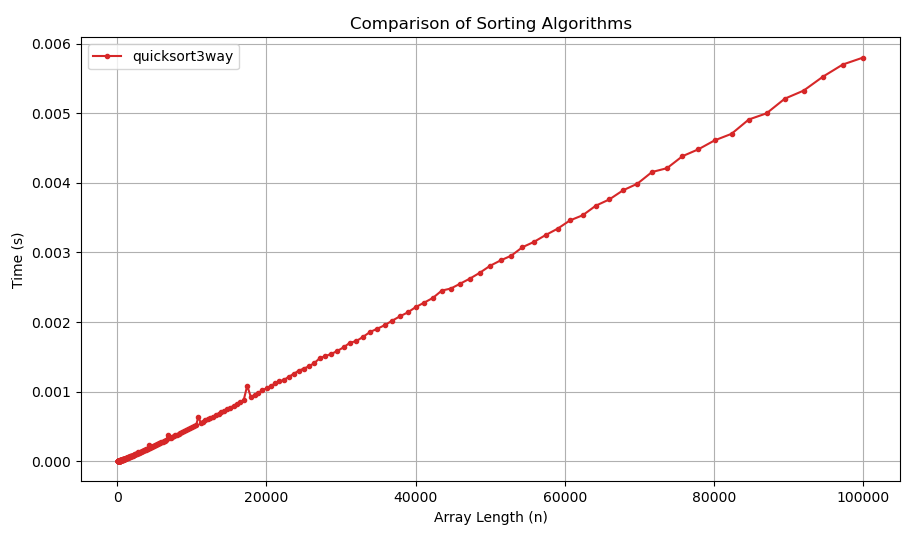
\includegraphics[width=0.6\textwidth]{Quicksort3way.png} \\
                %\vspace{0.5cm}
                \textbf{Grafico.9} Grafico in scala lineare\\
                \vspace{0.5cm}
                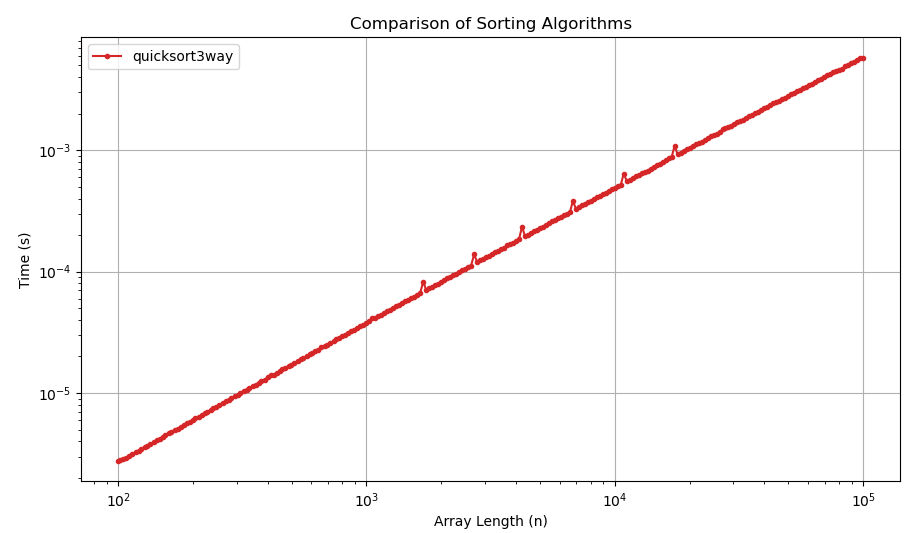
\includegraphics[width=0.6\textwidth]{Quicksort3way_Log.png} \\
                %\vspace{0.5cm}
                \textbf{Grafico.10} Grafico in scala logaritmica\\
            \end{center}
            Come per il quicksort standard, il comportamento dell'algoritmo al variare di $n$ non presenta particolari discrepanze con l'analisi asintotica.

        \subsubsection{Grafici al variare di \textit{m}}
            \begin{center}
                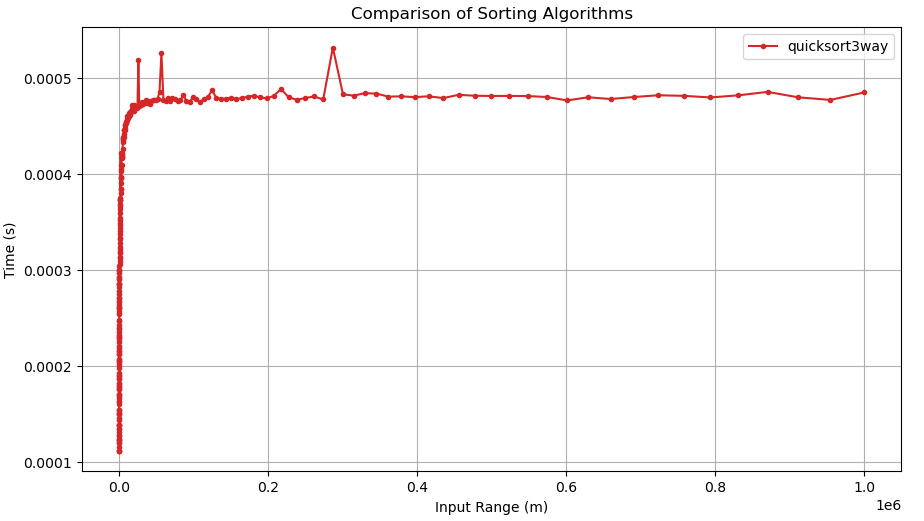
\includegraphics[width=0.6\textwidth]{QuickSort3way_InputRange.png} \\
                %\vspace{0.5cm}
                \textbf{Grafico.11} Grafico in scala lineare\\
                \vspace{0.5cm}
                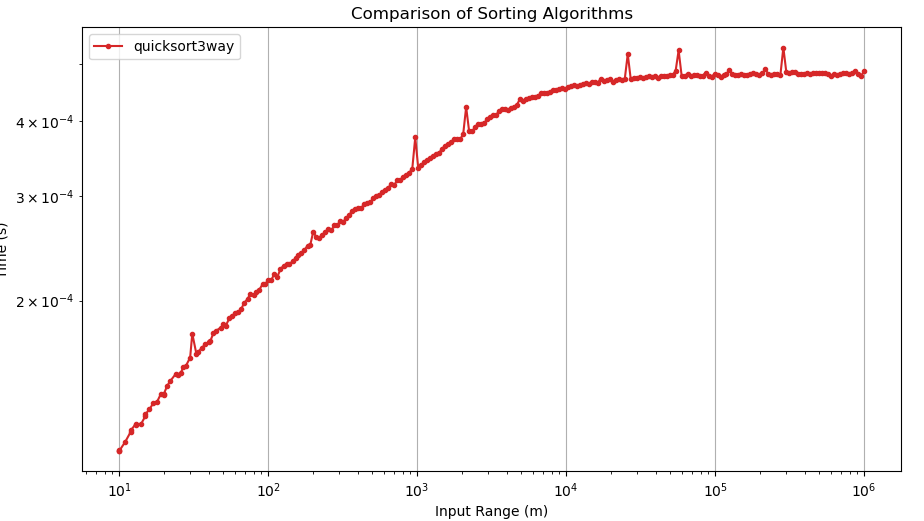
\includegraphics[width=0.6\textwidth]{QuickSort3way_InputRange_Log.png} \\
                \textbf{Grafico.12} Grafico in scala logaritmica\\
            \end{center}
            La procedura partition modificata in modo da dividere il vettore in tre parti e dedicarne una per gli elementi uguali al perno rende quicksort 3 way molto efficiente quando si trattano vettori con range di input molto piccolo, rendendo quicksort3way più efficiente di quicksort sotto questo punto di vista. Addirittura, come si può infatti notare dai grafici, il tempo migliore si è registrato per il valore $m$ più basso, per poi aumentare rapidamente al crescere della differenza nel range, fino a stabilizzarsi da $m=10^4$ in poi.

    \subsection{Countingsort}
        \subsubsection{Grafici al variare di \textit{n}}
            \begin{center}
                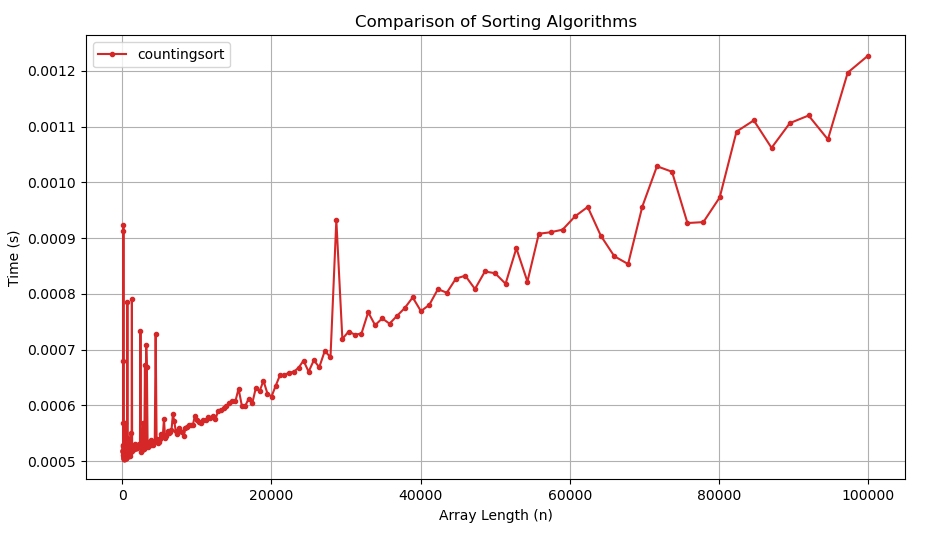
\includegraphics[width=0.6\textwidth]{Countingsort.png} \\
                %\vspace{0.5cm}
                \textbf{Grafico.5} Grafico in scala lineare\\
                \vspace{0.5cm}
                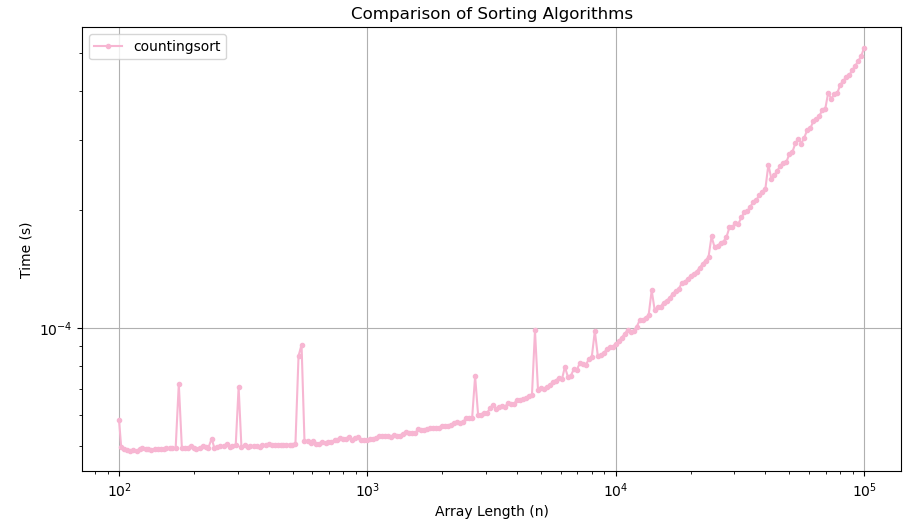
\includegraphics[width=0.6\textwidth]{Countingsort_Log.png} \\
                %\vspace{0.5cm}
                \textbf{Grafico.6} Grafico in scala logaritmica\\
            \end{center}
            Il comportamento dell'algoritmo al variare di $n$ non presenta particolari discrepanze con l'analisi asintotica.
            
        \subsubsection{Grafici al variare di \textit{m}}
            \begin{center}
                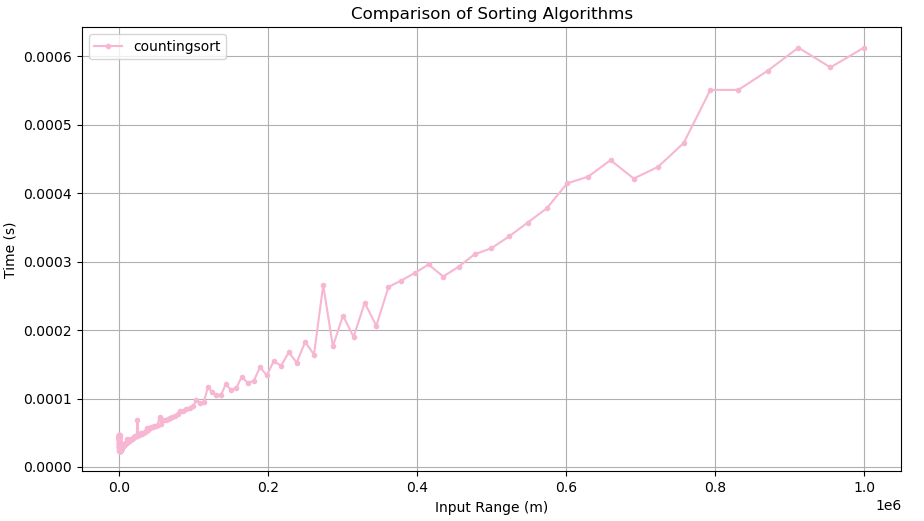
\includegraphics[width=0.6\textwidth]{Countingsort_InputRange.png} \\
                %\vspace{0.5cm}
                \textbf{Grafico.7} Grafico in scala lineare\\
                \vspace{0.5cm}
                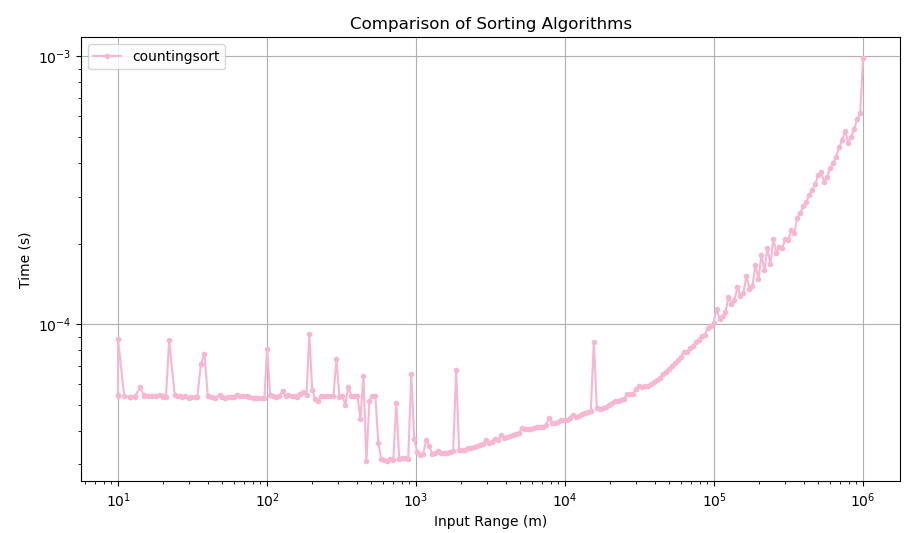
\includegraphics[width=0.6\textwidth]{Countingsort_InputRange_Log.png} \\
                \textbf{Grafico.8} Grafico in scala logaritmica\\
            \end{center}
            Come ci si aspettava dal calcolo asintotico, per valori $m$ piccoli, counting sort si comporta in meglio.
    
    \subsection{Introsort}
        \subsubsection{Grafici al variare di \textit{n}}
            \begin{center}
                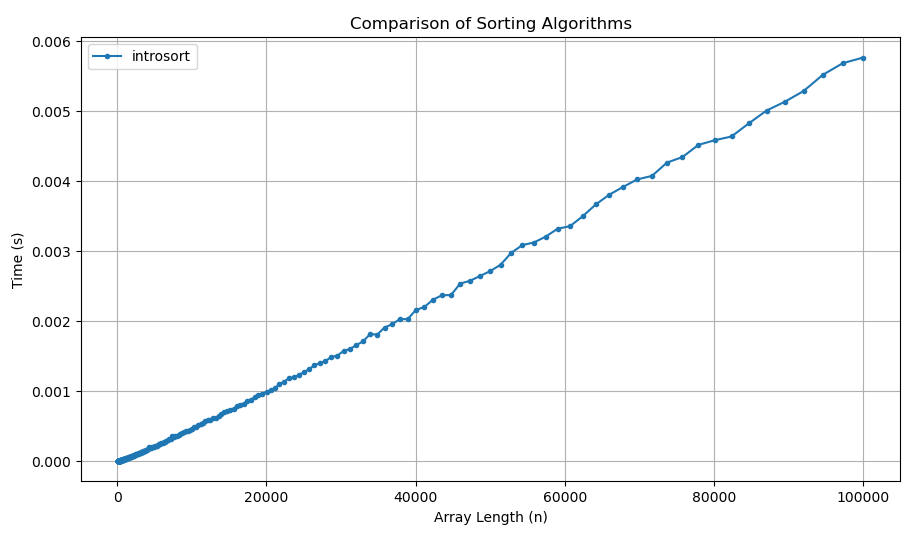
\includegraphics[width=0.6\textwidth]{Introsort.png} \\
                %\vspace{0.5cm}
                \textbf{Grafico.13} Grafico in scala lineare\\
                \vspace{0.5cm}
                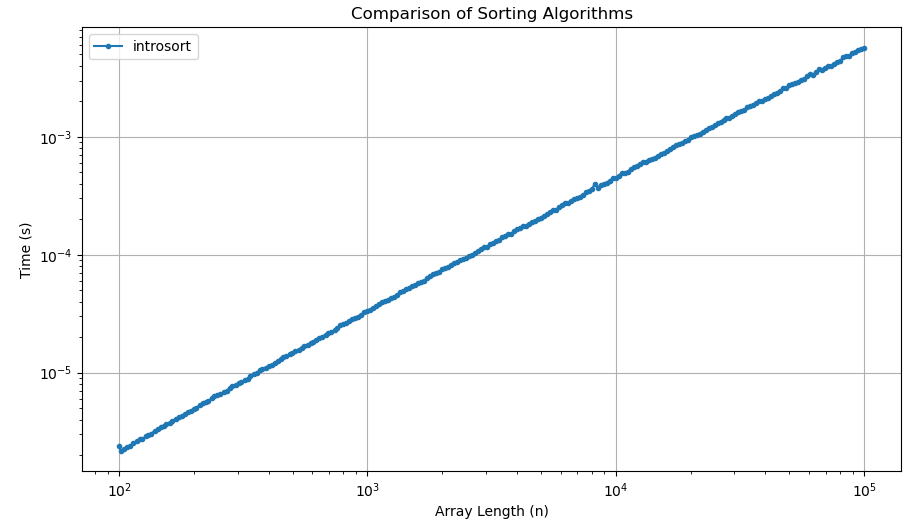
\includegraphics[width=0.6\textwidth]{Introsort_Log.png} \\
                %\vspace{0.5cm}
                \textbf{Grafico.14} Grafico in scala logaritmica\\
            \end{center}
            Il comportamento dell'algoritmo al variare di $n$ non presenta particolari discrepanze con l'analisi asintotica.

        \subsubsection{Grafici al variare di \textit{m}}
            \begin{center}
                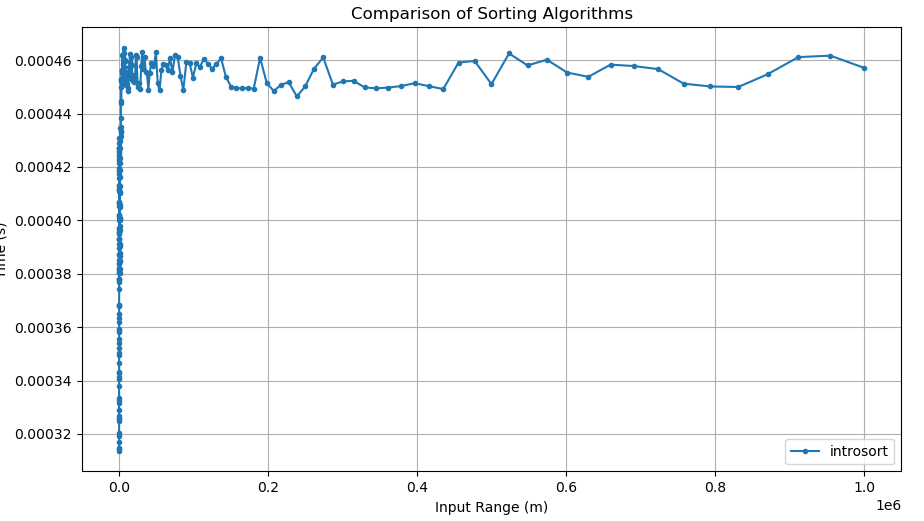
\includegraphics[width=0.6\textwidth]{Introsort_InputRange.png} \\
                %\vspace{0.5cm}
                \textbf{Grafico.15} Grafico in scala lineare\\
                \vspace{0.5cm}
                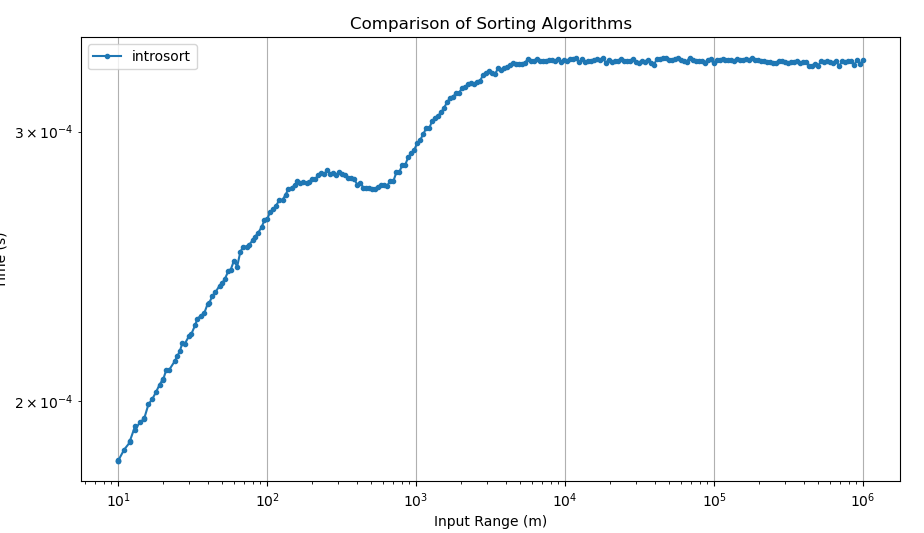
\includegraphics[width=0.6\textwidth]{Introsort_InputRange_Log.png} \\
                \textbf{Grafico.16} Grafico in scala logaritmica\\
            \end{center}
            Come si può notare, specialmente nella visualizzazione con scala asintotica, l'algoritmo sembra comportarsi meglio con $m$ basso. Questo è riconducibile all'implementazione di heapsort, in quanto avere molti valori simili in una heap, può tendere ad abbassarne il costo di operazione.
            
    \subsection{Confronto tra gli algoritmi}
        \subsubsection{Grafici al variare di \textit{n}}
            \begin{center}
                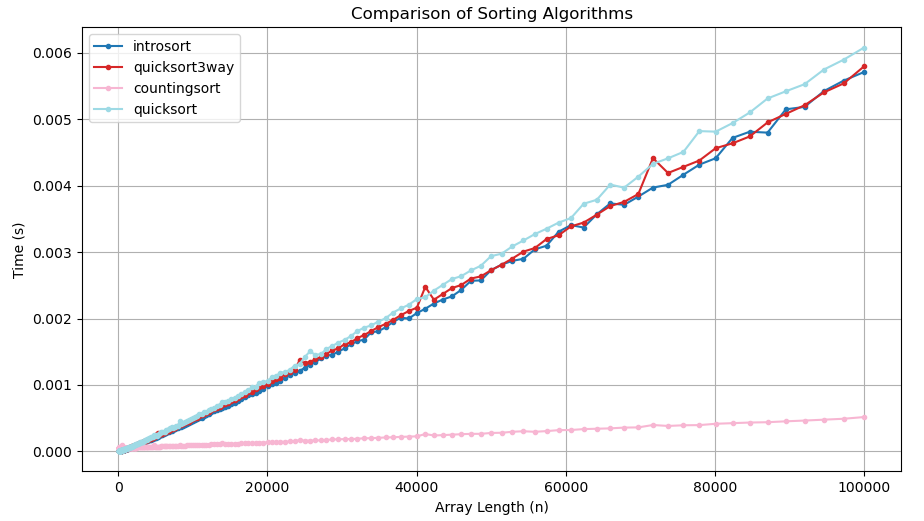
\includegraphics[width=0.6\textwidth]{Tutti.png} \\
                %\vspace{0.5cm}
                \textbf{Grafico.17} Grafico in scala lineare\\
                \vspace{0.5cm}
                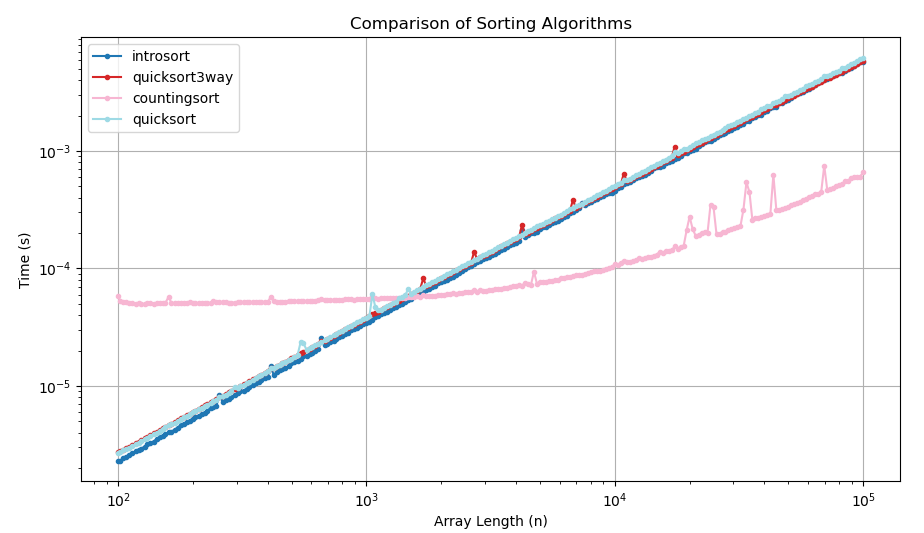
\includegraphics[width=0.6\textwidth]{Tutti_Log.png} \\
                \textbf{Grafico.18} Grafico in scala logaritmica\\
                \vspace{0.5cm}
            \end{center}
            Come si può osservare da questi grafici di confronto, countingsort è meno efficiente rispetto agli altri tre algoritmi, nel caso di vettori di lunghezza fino a poco più di 1'000 elementi.
            
            Tuttavia man mano che ci si allontana dalla soglia dei 1'000 elementi, il tempo impiegato da countingsort cresce molto meno rispetto agli altri algoritmi.

            Notiamo infatti che la cresita di countingsort è lineare, tuttavia gli altri tre hanno andamento $\Theta(nlog(n))$, quindi la performance per $n$ grandi è giustificata.\\
            Come è possibile però giustificare l'andamento per $n$ piccolo? Ricordiamo che countingsort ha costante moltiplicativa molto alta, quindi per piccoli $n$, la quest'ultima prende il sopravvento sul costo asintotico, rendendo quindi le esecuzioni lunghe.

            Notiamo inoltre che si possono osservare delle perturbazioni in alcuni punti dei grafici. Queste ultime non dipendono dall'algoritmo, ma da fattori esterni e fuori dal nostro controllo, come la cache o lo scheduling del sistema operativo.

        \subsubsection{Grafici al variare di \textit{m}}
            \begin{center}
                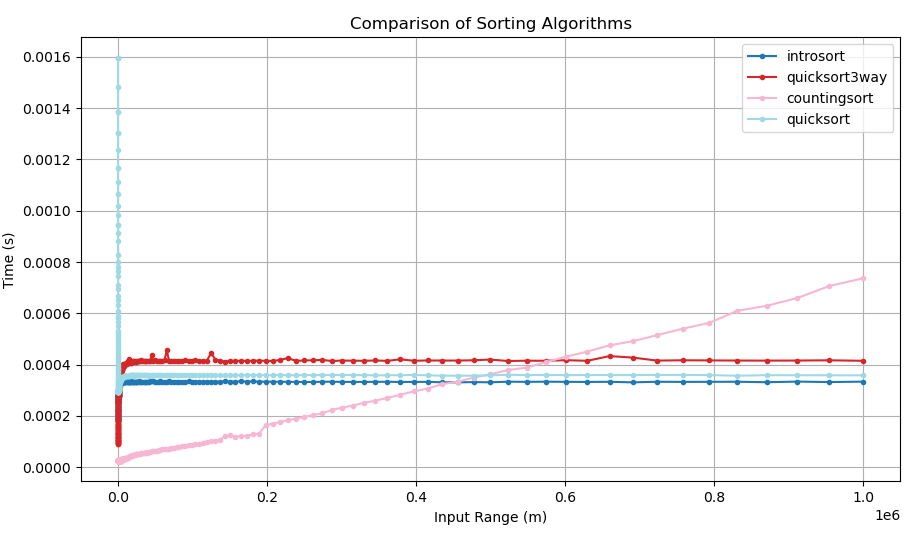
\includegraphics[width=0.6\textwidth]{Tutti_InputRange.png} \\
                %\vspace{0.5cm}
                \textbf{Grafico.19} Grafico in scala lineare\\
                \vspace{0.5cm}
                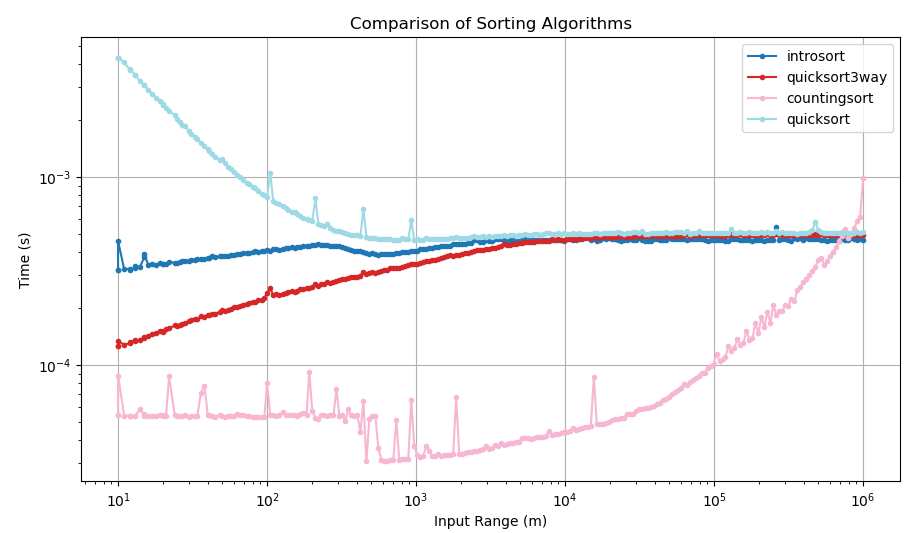
\includegraphics[width=0.6\textwidth]{Tutti_InputRange_Log.png} \\
                \textbf{Grafico.20} Grafico in scala logaritmica\\
                \vspace{0.5cm}
            \end{center}
            Dai due grafici, in particolare dal secondo, si può vedere che per piccole differenze nel range, countingsort si conferma il migliore algoritmo.
            
            Tuttavia, al crescere delle differenze nel range di input, countingsort continua ad aumentare il tempo impiegato, mentre gli altri algoritmi sembrano stabilizzarsi, dunque sembra che per differenze di range maggiore, countingsort venga superato dagli altri tre, o per lo meno eguagliato.

            Osserviamo, come detto in precedenza che per piccoli $m$, quicksort risulta inferiore.

\section{Confronto Tra Hardware}
    Si osservino i seguenti grafici, generati con la stessa implementazione del runner e con gli stessi parametri su piattaforme diverse.

    \begin{center}
        \includegraphics[width=0.6\textwidth]{Github_Tutti.png} \\
        \textbf{Figura.11} Gli algoritmi eseguiti come action su github\\
        \vspace{0.2cm}
        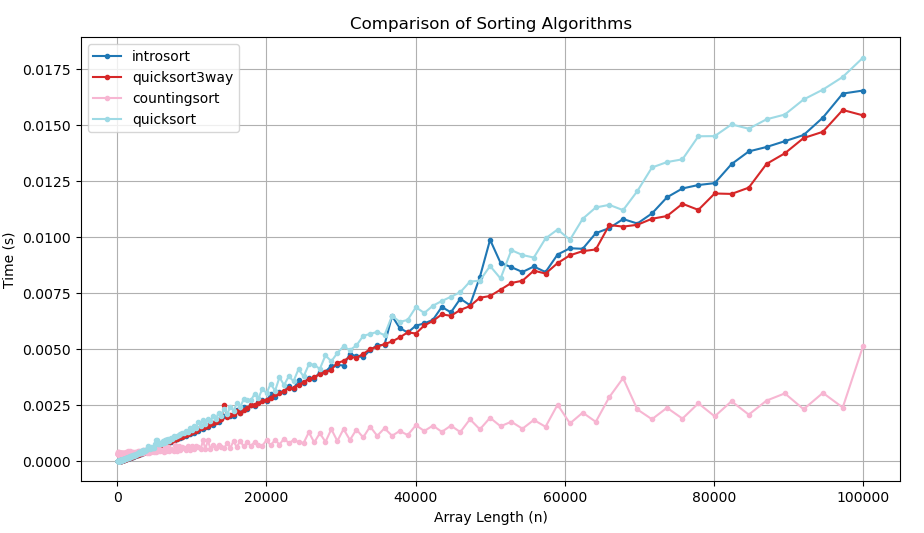
\includegraphics[width=0.6\textwidth]{Filippo_Tutti.png} \\
        \textbf{Figura.12} Gli algoritmi eseguiti sul computer di Filippo (Dell Vostro 15-3568 CPU: Intel Core i5 7th Gen - 2016)\\
        \vspace{0.5cm}
        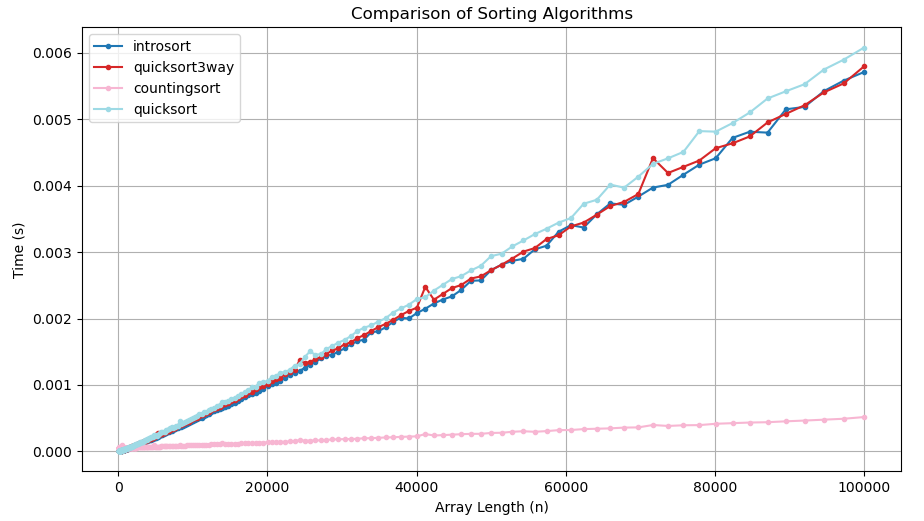
\includegraphics[width=0.6\textwidth]{Tutti.png} \\
        \textbf{Figura.13} Gli algoritmi eseguiti sul computer di Francesco (MacBook Air M2 - 2022)\\
    \end{center}

    Notiamo innanzitutto che anche la stabilità degli algoritmi cambia tra piattaforme. Si osservi nel particolare il grafico relativo al \textit{Macbook} di Francesco, utilizzante hardware \textit{arm} e sistema operativo \textit{MacOs}. Notiamo che i risultati sono veramente stabili.
    Una speculazione alla motivazione di ciò è che il clock di \textit{MacOs} ha risoluzione molto bassa: è addirittura fino a 10 volte meno preciso del clock fornito da linux, sebbene il codice relativo alla misurazione sia lo stesso. Questo causa un numero molto più alto di esecuzioni necessarie per ottenere l'errore minimo relativo desiderato. La conseguenza sarebbero, paradossalmente, risultati più stabili.

    Successivamente è necessario osservare che gli algoritmi che risultano i più efficienti in una macchina non lo sono anche per l'altra: ad esempio nel computer di Filippo, il quicksort 3 way risulta più efficiente dell'introsort, mentre nel calcolatore di Francesco risulta più efficiente l'introsort. Addirittura la generazione dei csv attraverso una \textit{GitHub Action} indicherebbe che i due siano equivalenti. Questo è dovuto a differenze sia software, come l'implementazione dello scheduler del sistema operativo, che hardware, come l'implementazione della cache e del numero di livelli.

    Constatiamo infine l'osservazione più importante e forse anche la più ovvia: i tempi di esecuzione non sono simili, tutt'altro. Il comportamento asintotico al variare di $n$ ed $m$ invece rimane lo stesso.

\section{Conclusioni}
    Sono stati analizzati gli algoritmi di ordinamento precedentemente elencati. È stato visto come il calcolo del costo asintotico si rispecchi sul tempo d'esecuzione per grandi $n$ e $m$, anche su macchine e sistemi operativi vari.

    Si è anche notato come per i piccoli numeri la costante moltiplicativa risulti più importante del costo asintotico: si ricordi il confronto tra quicksort e countingsort per $n$ piccoli.

    Si può concludere dicendo che l'intero progetto è stato un'interessante analisi sul costo e sulla performance di algoritmi nel mondo reale. Gli insegnamenti appresi da questo progetto resteranno sicuramente utili per scrivere software performante nel futuro.

\end{document}
